\chapter{Demand Decides Your Price}

The obvious answer is not always the useful answer.

Ask what determines the price of your time, and many people will immediately say, ``my value.'' That answer is not wrong, but it is incomplete in a dangerous way. A person can become more capable, more diligent, and more expensive to train, and still find that the world refuses to pay much for his time.

The missing word is demand.

\begin{quote}
In a market, the most important factor deciding price is demand.
\end{quote}

This is one of those ideas everyone seems to know until the exact moment when it is needed. We know it when buying goods, but forget it when thinking about our own work. We know it in economics, but forget it in love, employment, writing, products, and personal ambition. Then we become resentful: I worked so hard. I gave so much. I paid such a high cost. Why does no one care?

The answer may be simple and painful:

\begin{quote}
The world did not need that thing enough.
\end{quote}

This chapter is not an argument against effort. It is an argument for aiming effort where need exists.

\section*{Forgetting the Main Thing}

People have a reliable talent for forgetting what matters most.

Every generation has its enthusiasms. There were radio enthusiasts, model airplane enthusiasts, personal computer enthusiasts, stereo enthusiasts, camera enthusiasts, and many more. Enthusiasm itself is not the problem. A life without enthusiasm is thin.

The problem appears when the tool replaces the purpose.

A stereo system is bought, supposedly, to hear music better. Yet many audio enthusiasts spend their best attention listening to glass shattering, aircraft explosions, gunfire, and other dramatic sound effects. A camera is bought to make better photographs, yet some owners spend more time comparing lenses than seeing the world. A computer is bought to work or create more efficiently, yet it easily becomes a machine for distraction. A phone is bought to connect with the world, yet many people use it to cut off real contact with the world.

The same mistake appears in work.

A person buys more tools, collects more certificates, spends more hours, makes more sacrifices, and assumes the market should reward the cost. But the buyer, employer, reader, user, partner, or investor is not mainly asking, ``How much did this cost you?'' The real question is:

\begin{quote}
Do I need this?
\end{quote}

If the answer is no, your cost does not create a price.

\section*{Cost Is Not Price}

Price and cost are related, but not directly and not completely.

A customer does not buy a product because the maker suffered. A reader does not owe attention because the writer spent many nights revising. A company does not pay a salary because the employee feels tired. A partner is not required to be moved because someone says, ``I gave so much.''

Before the buyer pays, the seller's cost belongs to the seller.

The buyer's decision is shaped mainly by need, alternatives, urgency, trust, and ability to pay. Cost may affect supply. It may affect whether the seller can continue. It may affect the minimum price the seller hopes to receive. But it does not, by itself, create demand.

\begin{center}
\begin{adjustbox}{max width=\linewidth}
\begin{tabular}{lll}
\hline
Confused view & Clearer view & Practical question \\
\hline
Cost decides price & Demand decides price & Who needs this? \\
Effort deserves reward & Usefulness earns reward & How useful is it? \\
My feeling matters most & The market has its own view & What does the world need? \\
\hline
\end{tabular}
\end{adjustbox}
\end{center}

If payment is made only because the buyer admires your sacrifice, it is closer to donation than purchase. There is nothing wrong with donation, but confusing donation with market exchange leads to bad decisions.

This confusion creates many ordinary disappointments. A person does things that are expensive to himself but not needed by others, then feels betrayed by the lack of response. The suffering was real. The conclusion was wrong.

The lesson is plain:

\begin{quote}
Do useful things. Make useful products. Become a useful person.
\end{quote}

Plain truths are easy to underestimate because they do not sound clever. Yet many lives change only when such a plain truth is finally obeyed.

\section*{The Demand Model}

The basic model is small enough to keep in memory:

\begin{center}
\begin{adjustbox}{max width=\linewidth}
\begin{tikzpicture}[node distance=1.1cm, every node/.style={font=\small}]
\node[draw, rounded corners, align=center, minimum width=2.6cm, minimum height=0.8cm] (need) {Demand};
\node[draw, rounded corners, align=center, minimum width=2.6cm, minimum height=0.8cm, right=of need] (value) {Perceived value};
\node[draw, rounded corners, align=center, minimum width=2.6cm, minimum height=0.8cm, right=of value] (price) {Price};
\node[draw, rounded corners, align=center, minimum width=2.6cm, minimum height=0.8cm, below=of value] (cost) {Your cost};
\draw[->] (need) -- (value);
\draw[->] (value) -- (price);
\draw[dashed, ->] (cost) -- (value);
\end{tikzpicture}
\end{adjustbox}
\end{center}

Your cost may support value, but it does not command price. Demand is the stronger force.

This matters for the price of your time. If you want a higher salary, the question is not merely, ``Have I worked hard?'' or ``Do I deserve more?'' A better question is:

\begin{quote}
Whose important demand can I satisfy better than the available alternatives?
\end{quote}

If you work for a boss, your salary is not primarily the result of your private sense of worth. It is the boss's willingness to pay for the problems you solve. If someone in your field already earns the income you want, study what demand he satisfies. What does he do that others cannot? What risk does he remove? What result does he reliably produce? What scarcity does he occupy?

If you run a product, the same rule applies. Users do not care about your internal drama. They care whether the product solves a problem they actually feel. A product can be elegant, sincere, and costly, yet weak, because too few people need it strongly enough.

\section*{Live Toward Future Demand}

Earlier we said that a good life is not merely ``living in the present.'' It is living with the future in view. Demand makes this instruction more concrete.

Before choosing a direction, ask:

\begin{enumerate}
\item How many people are likely to need this in the future?
\item How strongly will they need it?
\item What value can I provide to them?
\item Will this need grow, shrink, or disappear?
\item What must I begin practicing now to serve that future need?
\end{enumerate}

A person who only reacts to present demand is always late. A person who can see future demand and start preparing now gains time. He does not need to predict perfectly. He only needs to aim better than those who never ask the question.

The rough picture is this:

\begin{center}
\begin{adjustbox}{max width=\linewidth}
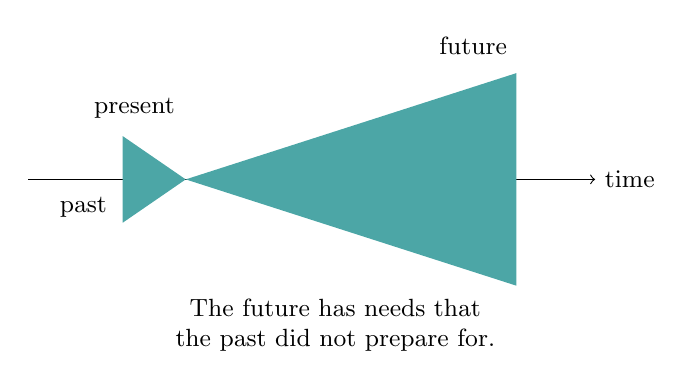
\begin{tikzpicture}[x=1cm,y=1cm,every node/.style={font=\small}]
\draw[->] (0,0) -- (7.2,0) node[right] {time};
\fill[teal!70] (1.2,-0.55) -- (2.0,0) -- (1.2,0.55) -- cycle;
\fill[teal!70] (2.0,0) -- (6.2,1.35) -- (6.2,-1.35) -- cycle;
\node at (0.7,-0.35) {past};
\node at (1.35,0.9) {present};
\node at (5.65,1.7) {future};
\node[align=center] at (3.9,-1.85) {The future has needs that\\the past did not prepare for.};
\end{tikzpicture}
\end{adjustbox}
\end{center}

Most people think from their own past: what they studied, what they like, what they have already done, what feels familiar. The market thinks from need. The future is especially indifferent to our past comfort.

This is why choice can matter more than effort. If the direction is wrong, more effort may only make the error more expensive.

\section*{Being Needed}

Strong connection with the world is one of the deepest sources of happiness.

This sounds sentimental until we describe it more clearly. The people who seem unusually happy are often people whose world genuinely needs them. Their family needs them. Their colleagues need them. Their users need them. Their readers need them. Their market needs them. Because they are needed, they are valued. Sometimes they are even overvalued.

This is not mysterious. It is demand at the human scale.

If you are the most useful person on a team, your compensation and treatment will tend to rise. If you are truly useful to a partner, not merely emotionally dramatic, you become hard to replace. If your product is the most useful tool for a large group of users, it spreads. QQ, WeChat, and Alipay became large on mobile devices not because users admired their internal cost, but because they were useful in daily life.

Being needed is difficult. If it were easy, more people would manage it.

The practice begins close to home. The world is not an abstraction; much of your world is made of the people around you. Ask, with names in mind:

\begin{enumerate}
\item What does my family most need?
\item What do my friends most need?
\item What does my boss most need?
\item What do my colleagues most need?
\item What do my partners most need?
\item What do my investors or customers most need?
\item What do they clearly not need?
\end{enumerate}

The last question is often the most efficient. When you know what others do not need, much useless speech and effort disappears.

\section*{A Better Form of Empathy}

Many people understand empathy as imagining one other person's feelings. That is useful, but too narrow.

For the purposes of wealth freedom, the stronger version is:

\begin{quote}
Learn to think from the position of the world.
\end{quote}

This means learning how groups of people think, choose, fear, pay, ignore, compare, and trust. One customer matters, but a category of customers matters more. One boss matters, but the structure of employer demand matters more. One reader matters, but the reader group matters more.

You can understand a person by working backward from his conclusions. If this is what he believes, what premises must he hold? If this is what he buys, what need does he feel? If this is what he ignores, what does he not value? The same reverse reasoning works on markets and societies.

This habit also reduces complaint. Much complaint comes from believing the world should match our private map. Mark Twain's warning is useful here: what gets a person into trouble is not only ignorance, but the discovery that the world is not as he imagined.

Demand-based thinking makes the world less personal. Other people's needs are theirs. Your needs are yours. They need not be identical. They often will not be identical. Once this is accepted, one appears more tolerant, not because of vague moral cultivation, but because the structure is clear.

For example, a person may believe astrology is useless. Yet many people read it, discuss it, and even use it to guide choices. Whether the need is real or imagined, demand exists. If you see this clearly, you do not need to waste attention hating astrology. It is enough to understand: other people are satisfying a need that is not yours.

Clear description often produces what people vaguely call good manners.

\section*{The Writing Example}

The previous chapter argued that writing is a reusable hour. This chapter adds the commercial and moral filter:

\begin{quote}
The writing must be useful.
\end{quote}

A writer can chase style, cleverness, elegance, structure, or personal expression. None of these is worthless. But if the reader's central demand is useful change, then decoration must serve usefulness or be removed.

This explains why useful writing may sometimes look plain. It may use fewer rhetorical tricks. It may repeat an important point until the reader actually understands it. It may sacrifice elegance to clarity. It may be accused of being too direct, too simple, or too repetitive. The question remains:

\begin{quote}
Does it help the reader change?
\end{quote}

If the answer is yes, the writing has value. If the answer is no, polished language only hides the absence of value.

The same filter applies to every product of attention. Before asking how to promote it, ask whether it is needed. Before asking how to charge for it, ask whom it helps. Before asking why the world has not rewarded you, ask whether you have made something the world has reason to reward.

\section*{Choosing What to Become}

There are many possible demands in the world. You do not have to satisfy all of them.

At one point, a person may notice that ``interesting people'' are often needed. The world likes entertaining people. Groups need someone who livens the room. Audiences reward wit. This is real demand.

But the next question is deeper:

\begin{quote}
Does this demand need to be satisfied by me?
\end{quote}

Being regarded as interesting and living an interesting life are not the same. In some cases, trying to perform the first may damage the second. If many people are already excellent at being publicly interesting, and if that role does not fit your deeper path, it may be wise to leave that demand to them.

Demand is not a command. It is information.

The best strategy is not ``do anything people want.'' That becomes servitude. The better strategy is:

\begin{quote}
Choose the most needed thing that you are willing and able to become excellent at serving.
\end{quote}

This choice joins market reality with personal direction. It prevents the arrogance of ignoring demand and the weakness of chasing every demand.

\section*{A Career Example}

When I first taught at New Oriental, I did not know immediately what would be most worthwhile to teach. Soon one fact became obvious: good teachers were always scarce, and good writing teachers were especially scarce. TOEFL writing, GRE writing, GMAT writing -- the demand was clear.

So the direction became clear. If I could teach writing well, I would become needed.

The work was concrete. I wrote model essays for the 185 TOEFL writing topics in the question bank, sometimes more than one version. I wrote every day, many pieces a day, for about half a year. The result was not only reputation. The result was rapid growth. I became the one person who had written through the whole bank.

The market responded predictably. Classes did not need to be begged for. They came. Others competed for teaching slots; I often needed to push them away to rest.

Later, when writing books, I taught reading and writing, but chose vocabulary books as a category. The reasoning was the same: choose where demand is strongest.

This example is not about one company or one exam. The principle is portable:

\begin{quote}
Find the shortage. Become capable there.
\end{quote}

\section*{The End of Useless Grievance}

One recurring sentence in life is:

\begin{quote}
I gave so much, and you were never moved.
\end{quote}

Sometimes the sentence describes real cruelty. But often it describes misdirected effort. The giver gave what was not needed, then demanded payment in gratitude.

A practical exercise can remove much bitterness. Write down your grievances. List the things you believe others failed to appreciate. Then examine each item with one question:

\begin{quote}
Was this actually needed by the other person?
\end{quote}

Some answers will be uncomfortable. That discomfort is useful. It returns attention from self-pity to reality.

This does not mean other people are always right. It does not mean all needs deserve obedience. It means that resentment is a poor substitute for understanding demand.

The road to wealth freedom requires repeated contact with reality. Attention must go where it can see. Capital must go where it can compound. Time must go where it can produce future choice. Effort must go where value is actually needed.

\section*{The Daily Question}

Because obvious truths are easily forgotten, they must become routine questions.

Ask daily:

\begin{enumerate}
\item Did I waste attention today?
\item Did I train metacognition today?
\item What is most important here?
\item Who needs what I am doing?
\item How strongly do they need it?
\item How can I make myself more useful?
\end{enumerate}

These questions are not ornamental. They are steering devices.

When you feel underpriced, ask what demand you satisfy. When you design a product, ask how many people need it and how urgently. When you choose a skill, ask whether future demand will reward it. When you help someone, ask what he actually needs. When you complain about the world, ask whether the world is different from your imagination.

The compact rule is worth writing plainly:

\begin{quote}
Choose the most needed thing worth doing.
\end{quote}

If you are doing what is most needed, and you can do it well, you become needed. The needed are often valued, sometimes overvalued, and rarely ignored for long. This is not sentiment. It is how price, opportunity, trust, and freedom begin to gather around a person.
